\subsection*{Change in mutations and neoantigens at recurrence}
Across our cohort of 115 samples from 93 donors, we identified 20,672 potential neoantigens, defined as mutated peptides predicted to bind autologous MHC class I with affinity $\leq 500$nm (Table \ref{tab:cohort}). All but 29 (0.14\%) neoantigens were private to a single donor.

To investigate changes in mutational burden and neoantigens associated with recurrence after treatment, we performed separate paired and unpaired analyses as well as a Bayesian regression integrating both paired and unpaired samples (Figure \ref{fig:bayesian}). The Bayesian analysis controls for tissue type (solid or ascites), sample purity, the number of samples from the same donor, and also probes an interaction between tissue type and recurrence. This model found that relapse, treated samples had 47\% (-2-125) more mutations, 49\% (-19-182) more neoantigens, and 104\% (2-300) more expressed neoantigens than primary samples.

\begin{table}
\begin{tabular}{llrrrlll}
\toprule
tissue type &  treatment &  donors &  samples &  samples with RNA &              Mutations &      Neoantigens & Expressed neoantigens \\
\midrule
    ascites &  untreated &       4 &        4 &                 4 &   10336 (9600 - 12000) &  205 (140 - 270) &         82 (50 - 110) \\
    ascites &    treated &      22 &       25 &                20 &  13757 (12000 - 15000) &  303 (260 - 350) &       149 (120 - 170) \\
      solid &  untreated &      75 &       75 &                69 &     7902 (7100 - 8900) &  166 (140 - 190) &          70 (58 - 83) \\
      solid &    treated &       9 &       12 &                 5 &   11250 (8500 - 14000) &  335 (220 - 460) &          41 (28 - 52) \\
\bottomrule
\end{tabular}
\caption{Cohort size and means.}
\label{tab:cohort}
\end{table}

\begin{figure}[h]
\centering
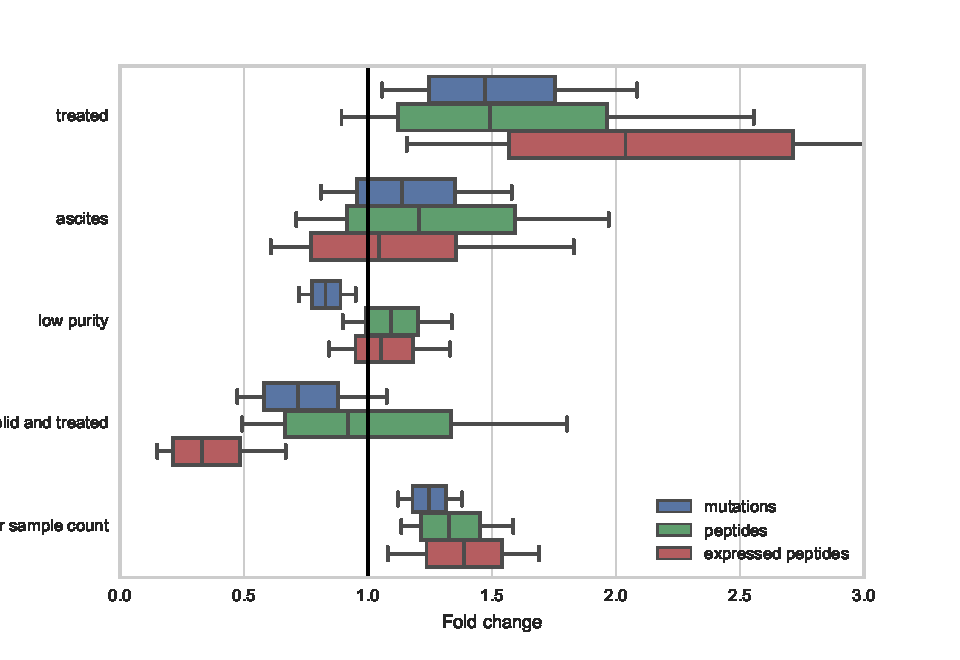
\includegraphics[scale=0.5]{figures/bayesian_model_effects.pdf}
\caption{Bayesian model effects. }
\label{fig:bayesian}
\end{figure}

\begin{itemize}
Peptides summary
\item We identified 25,920 distinct neoantigens, of which 9,506 had evidence for RNA expression ($>2$ variant-supporting RNA reads). All but 63 (0.24\%) neoantigens were unique to a single donor. For frameshift mutations, we considered all peptides generated until a stop codon. Single nucleotide variants, multinucleotide variants, and small insertions and deletions, accounted for 79\%, 12\%, and 9\% of the neoantigens, respectively.

Recurrence samples have more peptides
\item 
\item In paired samples, increase in total mutations (11/12 donors, $p=.01$, binomial test), increase in predicted MHC I binding mutant peptides (10/12, $p=.04$), and trend toward more expressed peptides (8/11 donors, $p=0.23$).  Mean increase in mutations was 62.1\% (bootstrap 95\% confidence interval 38.6-87.4), peptides 35.7\% (16.6-54.3), and expressed peptides 76.0\% (120.9-237.8).
\item As sample type is a confounding variable we additionally performed an unpaired analysis (figure 2) stratified by sample tissue type (solid or ascites). Summarized in table. All samples showed trend toward more mutatinos and peptides. For ascites, significant increase in expressed peptides, and for solid a significant increase in peptides. Interestingly, there was a significant *decrease* in expressed peptides among the solid tumors, despite an increase in overall peptides in the genome, when comparing the 69 untreated solid samples with RNA to the 5 treated samples with RNA.  This is consistent with a model in which solid tumors downregule expression of neoantigens after chemo exposure in response to treatment-induced immune infiltration. In untreated solid tumors, 43\% (40-46) of peptides have expression, whereas only 20\% (11-32) of the treated solid tumors. However, this change did not reach significance ($p-0.16$). In contrast, ascites samples saw a significant increase from 37\% (30-43) to 49\% (45-54) ($p=.046$). This is consistent with the idea that solid tumors are under immune surveillence whereas ascites are not. However, 4/5 of the treated samples with RNA are neoadjuvant chemo treated primary samples, so confounding due to which patients are selected for neoadjuvant chemo is also possible.

% ; the single recurrence sample (AOCS-094-2) had more expressed peptides (75) than any of the other four samples
% This was in turn signifincantly less than overall treated and untreated primary solid samples ($p=.003$).

\item consider bayesian model?

Sources of the increase in peptides


\item peptides per mutation?
\item Is mutation rate alone accounting for increase or does kind of mutation (indels) affect it?

\item Deconvolution of unique to treated mutations attributes no mutations to platinum signature
\item Number of peptides attributed to each signature
\end{itemize}

The Australian Ovarian Cancer Study (AOCS)\cite{Patch_2015} performed whole genome sequencing on 92 high grade serous Ovarian cancer tumors, including 15 donors with matched primary and acquired resistance samples. Their analysis found that the recurrence samples harbored more somatic mutations than the primary samples and were enriched for mutations in a $C(C \gt T)C$ context, suggestive of a possible impact of chemotherapy. We extend this analysis by quantifying the number of potential neoantigen-generating mutations in the primary and recurrence samples and testing whether mutational signature deconvolution attributes the unique-to-recurrence mutations to the \texit{C. Elegans} cisplatin signature. We include three additional donors from TCGA and one donor from our institution in our analysis (\ref{tab:cohort}).

Bulk comparison of treated and untreated samples stratified by tissue type (solid or ascites) and study cohort (AOCS, TCGA, or PT189) found no significant change in total mutations, neoantigens, or expressed neoantigens between pre-treatment and post-treatment samples (\ref{fig:unpaired}). We therefore focused on paired comparison of the 16 donors with both pre- and post-treatment samples available. 

As surgery is not usually performed for relapsed disease, the AOCS relapsed samples consist predominantly of drained ascites samples. We analyze ascites separately from solid tumors to avoid confounding. 


Intrinsic differences between solid tumor samples and ascites are a potential confounder for these analyses, so we analyze 

consists 

\section*{Neoantigen counts}


Here we analyze the neoantigen burden burden of these paired tumors 

The relapse samples contain on average 27\% (range -17\% to 134\%) more detected somatic mutations than the matched primary samples. The number of potential neoantigens increased accordingly from a mean of XX in the primary samples to XX at relapse. The new mutations undetected in the primary samples tended to be found at lower variant allele frequency (VAF) in the relapse samples than shared mutations (Mann-Whitney $p \lt .01$ in 14/16 samples), indicating the new mutations tended to be more subclonal. However, the size of this effect was relatively small. On average the mutations private to the relapse sample were found at 82\% ( 95\% CI=72-93) of the VAF of shared mutations. This effect was smaller still for mutations predicted to bind MHC I. Within this subset, new mutations were found at 89\% (72-107) of the VAF of shared mutations.

To explore possible etiologies for the increased mutational burden at recurrence, we deconvolved the mutations present in the primaries as well as the unique-to-recurrence mutations into known signatures. We used the 30 signatures curated by COSMIC (http://cancer.sanger.ac.uk/cosmic/signatures) plus an additional signature manually extracted from a study of cisplatin-exposed \textit{C. Elegans} [Meier et al]. Consistent with results originally reported by Patch et al on the AOCS cohort, the mutations were attributable mostly to Signatures 1 and 3, which are associated with Age and BRCA disruption, respectively. These two signatures together accounted for 82\% (75-88) of the mutations in primary samples and 70\% (64-76) of the mutations unique to the relapses. The remaining mutations in the relapses were attributed to different signatures in various samples. Signature 4, associated with smoking, was the only additional signature consistently given nonzero weight in the relapse samples. In the 9 relapse samples in which it was assigned nonzero weight, Signature 4 accounted for 10\% (8-13) of the unique-to-relapse mutations. Two primary samples also showed evidence for Signature 4. Smoking history of these patients was not known.

This suggests the increased burden at relapse in these Ovarian cancer samples is not predominantly due to direct mutagenic impact of the adjuvant chemotherapy, in contrast to a recent report for neo-adjuvant treated Esophageal cancer.
 
The signature contributions to the primary tumors were not significantly different between high-VAF and low-VAF mutations, suggesting that the mutagenic processes at work in the primary samples were not undergoing change at the time of primary surgery. The decrease in mutations attributable to Signatures 1 and 3 in the unique-to-relapse mutations is therefore potentially an indication of a therapy-driven shift. However, 

We note that the C(C>T)C mutations found at higher rates in the relapse samples do not correspond to the signature found in \textit{C. Elegans} (supplementary figure)


\iffalse

\section*{Introduction}




\section*{Results}
\subsection*{Somatic mutation and neoantigen burden}

As previously reported for the AOCS patients, there were significantly more detectable somatic mutations in the relapse samples over matched primary samples (increase in 15/16 sample pairs; binomial test $p \lt 0.001$). The change ranged from -17\% to 134\% with a mean of 27\%.

We considered the number of mutations resulting in peptides predicted to bind autologous class I MHC with 500nm or stronger affinity (figure \ref{fig:mhc_binding_mutations}). In accordance with the increase in overall mutation burden, we observed an upward trend in potential neoantigens at recurrence. For 10/14 patients, relapse samples harbored more potential neoantigens than matched primary samples; however this trend did not reach significance (p=0.18). The change ranged from -27\% to 126\% with a mean of 29\%. About half of these mutations had evidence for expression in the RNA-seq. For 9/13 donors the number of expressed potentially antigenic mutations increased at relapse (-53\% -- 407\%, mean 18\%) (p=0.27) (figure \ref{fig:expressed_mhc_binding_mutations}). We found no evidence for selection against expressed potential neoantigens at relapse (data not shown).

TODO: results bayesian model that includes therapy and basic patient info to predict number of mutations

% As expected somatic mutation and neoantigen burden were highly correlated with no substantial deviations
% Therapy vs. burden

\subsection*{Clonality}
Most of our primary tumors are solid and most of the relapse are ascites, making it challenging to directly address changes in clonality during the time of treatment. We instead focus on the relapse samples and compare the allelic fractions of private vs. shared mutations.

TODO: sciclone / pyclone / phylowgs number of clones (or entropy of clones?) comparing pre-vs-post treatment

The new mutations undetected in the primary samples tended to be found at lower variant allele frequency (VAF) in the relapse samples than shared mutations (Mann-Whitney $p \lt .01$ in 14/16 samples), indicating the new mutations tended to be more subclonal. However, the size of this effect was relatively small. On average the mutations private to the relapse sample were found at 82\% (bootstrap 95\% CI=72-93) of the VAF of shared mutations. This effect was smaller still for mutations predicted to bind MHC I. Within this subset, new mutations were found at 89\% (72-107) of the VAF of shared mutations.

\subsection*{Mutation signatures}
To explore possible etiologies for the increased mutational burden at recurrence, we deconvolved the mutations present in the primaries as well as the unique-to-recurrence mutations into known signatures. We used the 30 signatures curated by COSMIC (http://cancer.sanger.ac.uk/cosmic/signatures) plus an additional signature manually extracted from a study of cisplatin-exposed \textit{C. Elegans} [Meier et al]. Consistent with results originally reported by Patch et al on the AOCS cohort, the mutations were attributable mostly to Signatures 1 and 3, which are associated with Age and BRCA disruption, respectively. These two signatures together accounted for 82\% (75-88) of the mutations in primary samples and 70\% (64-76) of the mutations unique to the relapses. The remaining mutations in the relapses were attributed to different signatures in various samples. Signature 4, associated with smoking, was the only additional signature consistently given nonzero weight in the relapse samples. In the 9 relapse samples in which it was assigned nonzero weight, Signature 4 accounted for 10\% (8-13) of the unique-to-relapse mutations. Two primary samples also showed evidence for Signature 4. Smoking history of these patients was not known.


\section*{Discussion}

The fraction of cancer cells harboring a neoantigen may be critical in its ability to be targeted by a T cell response \cite{McGranahan_2016}.

\section*{Limitations}
RNA with hard thresholds to detect expressed peptides is subject to confounding by changes in gene expression -- e.g. if something gets upregulated post treatment





